\documentclass{article}
\usepackage[margin=1in,letterpaper]{geometry}
\usepackage{amsmath,amsfonts,amssymb,amsthm}
\usepackage{graphicx}

% For source code
\usepackage{listings}

% Algorithms and pseudocode
\usepackage[linesnumbered,ruled,vlined]{algorithm2e}
\usepackage{algpseudocode}

% Common shortcuts
\newcommand{\round}[1]{\lfloor {#1} \rceil}
\newcommand{\Norm}[1]{\Vert {#1} \Vert}
\newcommand{\norm}[1]{\vert {#1} \vert}
\newcommand{\var}[1]{\operatorname{Var}[{#1}]}
\newcommand{\leftsample}{\overset{{\scriptscriptstyle\$}}{\leftarrow}}

% Environments: definitions, theorems, propositions, corollaries, lemmas
%    Theorems, propositions, and definitions are numbered within the section
%    Corollaries are numbered within the theorem, though they are rarely used
\newtheorem{definition}{Definition}[section]
\newtheorem{theorem}{Theorem}[section]
\newtheorem*{remark}{Remark}
\newtheorem{corollary}{Corollary}[theorem]
\newtheorem{proposition}{Proposition}[section]
\newtheorem{lemma}{Lemma}[theorem]


\title{ECE 612, Information Theory}
\author{Ganyu (Bruce) Xu (g66xu)}
\date{Winter, 2024}

\begin{document}
%%%% TITLE %%%%%
% \maketitle

\section*{Preliminares}
    \begin{definition}
        The normal distribution $N(\mu, \sigma^2)$ has the probability density function

        $$
        f(x) = \frac{1}{\sigma\sqrt{2\pi}}\exp(-\frac{1}{2}(\frac{x-\mu}{\sigma})^2)
        $$
    \end{definition}

    \begin{definition}
        The joint normal distribution $N(\mathbf{\mu}, K)$ is defined by probability density function:

        $$
        f(\mathbf{x}) = \frac{1}{\sqrt{(2\pi)^n\det(K)}}
        \exp(-\frac{1}{2}
            (\mathbf{x} - \mathbf{\mu})^\intercal
            K^{-1}
            (\mathbf{x} - \mathbf{\mu})
        )
        $$
    \end{definition}

    \begin{theorem}[Joint normality implies marginal normality]
        If $\mathbf{X} = (X_1, X_2, \ldots, X_n)$ follows a joint normal distribution, then any linear combination of $\mathbf{X}$ follows normal distribution.
    \end{theorem}

\section{Entropy, mutual information, divergence}
    \begin{definition}[Entropy]
    The entropy of a random variable $X \in \mathcal{X}$ is defined by

        \begin{equation*}
            H(X) = -\sum_{x \in \mathcal{X}}p_X(x)\log{p_X(x)}
        \end{equation*}
    \end{definition}

    \begin{definition}[KL Divergence]
        The \textbf{KL Divergence} between two probability distributions $p, q$ on the same support $\mathcal{X}$ is defined by

        \begin{equation*}
            D(p \Vert q) = \sum_{x \in \mathcal{X}} p(x) \log{
                \frac{p(x)}{q(x)}
            }
        \end{equation*}
    \end{definition}

    \begin{definition}[Mutual information]
        The mutual information between two random variables $X, Y$ is defined by

        \begin{equation*}
            I(X; Y) = H(X) - H(X \mid Y)
        \end{equation*}

        It can also be expressed as the KL divergence between the joint distribution $p_{X, Y}$ and the product of marginal distribution $p_Xp_Y$:

        \begin{equation*}
            I(X; Y) = D(p_{X,Y} \Vert p_X \cdot p_Y)
        \end{equation*}
    \end{definition}

    \begin{proposition}
    Conditioning does not increase entropy
        \begin{equation*}
            H(X \mid Y) \leq H(X)
        \end{equation*}
    \end{proposition}

    A nice trick for reasoning about the entropy of "sum of random variables":

    $$
    \begin{aligned}
        H(X + Y \mid X) &= \sum_{x \in \mathcal{X}}p_X(x)H(X + Y \mid X=x) \\
        &= \sum_{x \in \mathcal{X}}p_X(x)H(x + Y \mid X=x) \\
        &= \sum_{x \in \mathcal{X}}p_X(x)H(Y \mid X=x) \\
        &= H(Y \mid X)
    \end{aligned}
    $$

    \subsection{Convexity}

    \begin{definition}
        A function $f$ is convex over the interval $x_1 \leq x \leq x_2$ if for all $0 \leq t \leq 1$:

        \begin{equation*}
            (1-t)f(x_1) + tf(x_2) \geq f((1-t)x_1 + tx_2)
        \end{equation*}
    \end{definition}

    Some notable functions' convexity:
    \begin{enumerate}
        \item Entropy is a concave function with respect to the probability distribution
        \item Mutual information $I(X; Y)$ is concave with respect to $p_X$ and is convex with respect to $p_{Y \mid X}$ for some fixed $p_X$
        \item $\log$ is a concave function
        \item The negative of a convex function is concave
        \item The sum or product of a linear function and a concave function is concave
        \item The composition of a linear function and a concave function is concave
    \end{enumerate}

    \begin{theorem}[Jensen's Inequality]
        If $f$ is a convex function and $X$ is a random variable, then
        \begin{equation*}
            E[f(X)] \geq f(E[X])
        \end{equation*}
    \end{theorem}

    \subsection{Markov chain}
    \begin{definition}
        Random variables $X, Y, Z$ form a Markove chain (denoted by $X \rightarrow Y \rightarrow Z$) if $p(z \mid x, y) = p(z \mid y)$
    \end{definition}

    \begin{theorem}[Data processing inequality]
        If $X \rightarrow Y \rightarrow Z$, then
        \begin{equation*}
            I(X; Z) \leq I(Y; Z)
        \end{equation*}
    \end{theorem}

    \begin{proposition}
        \begin{equation*}
            I(X; Y \mid Z) = 0 \Leftrightarrow X \rightarrow Z \rightarrow Y
        \end{equation*}
    \end{proposition}

    \begin{proposition}
        If $X \rightarrow Y \rightarrow Z$, then $Z \rightarrow Y \rightarrow X$
    \end{proposition}

    \begin{theorem}
        Let $X, Y$ be random variables. $I(X; Y)$ is concave with respect to the probability distribution of X. For a fixed marignal distribution of $X$, $I(X; Y)$ is convex with respect to $f_{Y \mid X}$
    \end{theorem}

    \begin{theorem}[Fano's inequality]\label{fanos-inequality}
        Let $X \rightarrow Y \rightarrow \hat{X}$ represent an encode-decode process, where $X, \hat{X} \in \mathcal{X}$ have the same support. Let $e$ denote decoding error $\hat{X} \neq X$, then:

        $$
        H(X \mid Y) \leq h(P_e) + P_e \log(\norm{\mathcal{X}})
        $$
    \end{theorem}

\section{Entropy rate}
    \begin{definition}
        A stochastic process is stationary if for all integer $n \geq 1$ and integer time shift (possibly negative) $l$:
        \begin{equation*}
            P[X_1^n] = P[X_{1+l}^{n+l}]
        \end{equation*}
    \end{definition}

    \begin{definition}
        A Markov chain is time invariant if for all $n \geq 1$:
        \begin{equation*}
            P[X_{n+1} \mid X_n] = P[X_2 \mid X_1]
        \end{equation*}
    \end{definition}

    \begin{definition}
        There are two definitions of entropy rate:
        \begin{enumerate}
            \item $H(\mathcal{X}) = \lim_{n\rightarrow\infty}\frac{1}{n}H(X_1^n)$
            \item $H^\prime(\mathcal{X}) = \lim_{n\rightarrow\infty}H(X_n\mid X_1^{n-1})$
        \end{enumerate}
    \end{definition}

    \begin{theorem}
        If $X_i$ is a stationary process, then the two entropy rates both exist and are equal
    \end{theorem}
    \begin{lemma}
        If $X_i$ is a stationary process, then $H(X_n \mid X_1^{n-1})$ is non-increasing with respect to $n$ and has a limit
    \end{lemma}

\section{Asymptotic equipartition property}
    \begin{theorem}[Weak law of large numbers (WLLN)]
        Let $X \sim p_X$ be a random variable, and let $X_l \sim p_X$ be i.i.d. random variables following the same distributions, then:

        \begin{equation*}
            \lim_{n \rightarrow \infty}\frac{1}{n}\sum_{i=1}^n X_i = E[X]
        \end{equation*}

        In other words, for any $\delta, \epsilon > 0$, there exists $N > 0$ such that for $n > N$:

        \begin{equation*}
            P[\norm{\frac{1}{n}\sum_{i=1}^n X_i - E[X]} < \delta] < \epsilon
        \end{equation*}
    \end{theorem}

    Recall that the entropy of a random variable can be defined as $H(X) = -E[\log(P_X)]$, so the weak law of large numbers also applies: the joint distribution of i.i.d. $X_i$ converges to the probability $2^{-nH(X)}$.

    \begin{definition}[Typical sequence]
        For random variable $X \sim p_X$, the set of \textbf{typical sequence} $A_\epsilon^n$ denotes the set of sequences whose probability is close to the entropy of the random variable

        \begin{equation*}
            A_\epsilon^{(n)} = \{
                \mathbf{x} \in \mathcal{X}^n 
                \mid \norm{
                    -\frac{1}{n}\log p_{\mathbf{X}}(\mathbf{x})
                    - H(X)
                } < \epsilon
            \}
        \end{equation*}
    \end{definition}

    \begin{theorem}[Asymptotic equipartition property]
        Let $X \sim p_X$ and let $\mathbf{X} \in \mathcal{X}^n$ denote i.i.d. sequence following the same distribution, then:

        \begin{enumerate}
            \item $\lim_{n \rightarrow \infty}P[\mathbf{X} \in A_\epsilon^{(n)}] = 1$
            \item $\norm{A_\epsilon^{(n)}} \leq 2^{n(H - \epsilon)}$
            \item For sufficiently large $n$, $\norm{A_\epsilon^{(n)}} \geq (1-\epsilon)2^{n(H+\epsilon)}$
        \end{enumerate}
    \end{theorem}

    \begin{proof}
        \textit{A sketch of the proof}
        (1) is the direct consequence of the weak law of large numbers

        (2): begin with \textbf{the sum of probability of all possible sequence is 1}

        (3): begin with \textbf{for sufficiently large $n$, $P[\mathbf{x} \in A_\epsilon^{(n)}] \geq 1 - \epsilon$}
    \end{proof}

\section{Data compressions}
    \begin{theorem}[Kraft inequality]
    A $D$-ary prefix code for a finite set of $m$ symbols $\mathcal{X}$ exists if and only if the lengths of the code words $l_1, l_2, \ldots, l_m$ satisfy:
    \begin{equation*}
        \sum_{x \in \mathcal{X}} D^{-l(x)} \leq 1
    \end{equation*}
    \end{theorem}

    Using the method of Lagrange multiplier, we can optimize the expected codeword length $E[L]$ under the constraint fo Kraft inequality:

    \begin{equation*}
        l_i = \lceil \log_D\frac{1}{p_i} \rceil
    \end{equation*}

    \begin{theorem}[Optimal code length]
    $H_D(X) \leq E[L] \leq H_D(X) + 1$
    \end{theorem}

    \begin{theorem}[McMillan inequality]
        A D-ary uniquely decodable code exists if and only if
        
        \begin{equation*}
            \sum_{i}D^{-l_i} \leq 1
        \end{equation*}
    \end{theorem}

    In practice, \textbf{Huffman code} offers the optimal noiseless compression:

    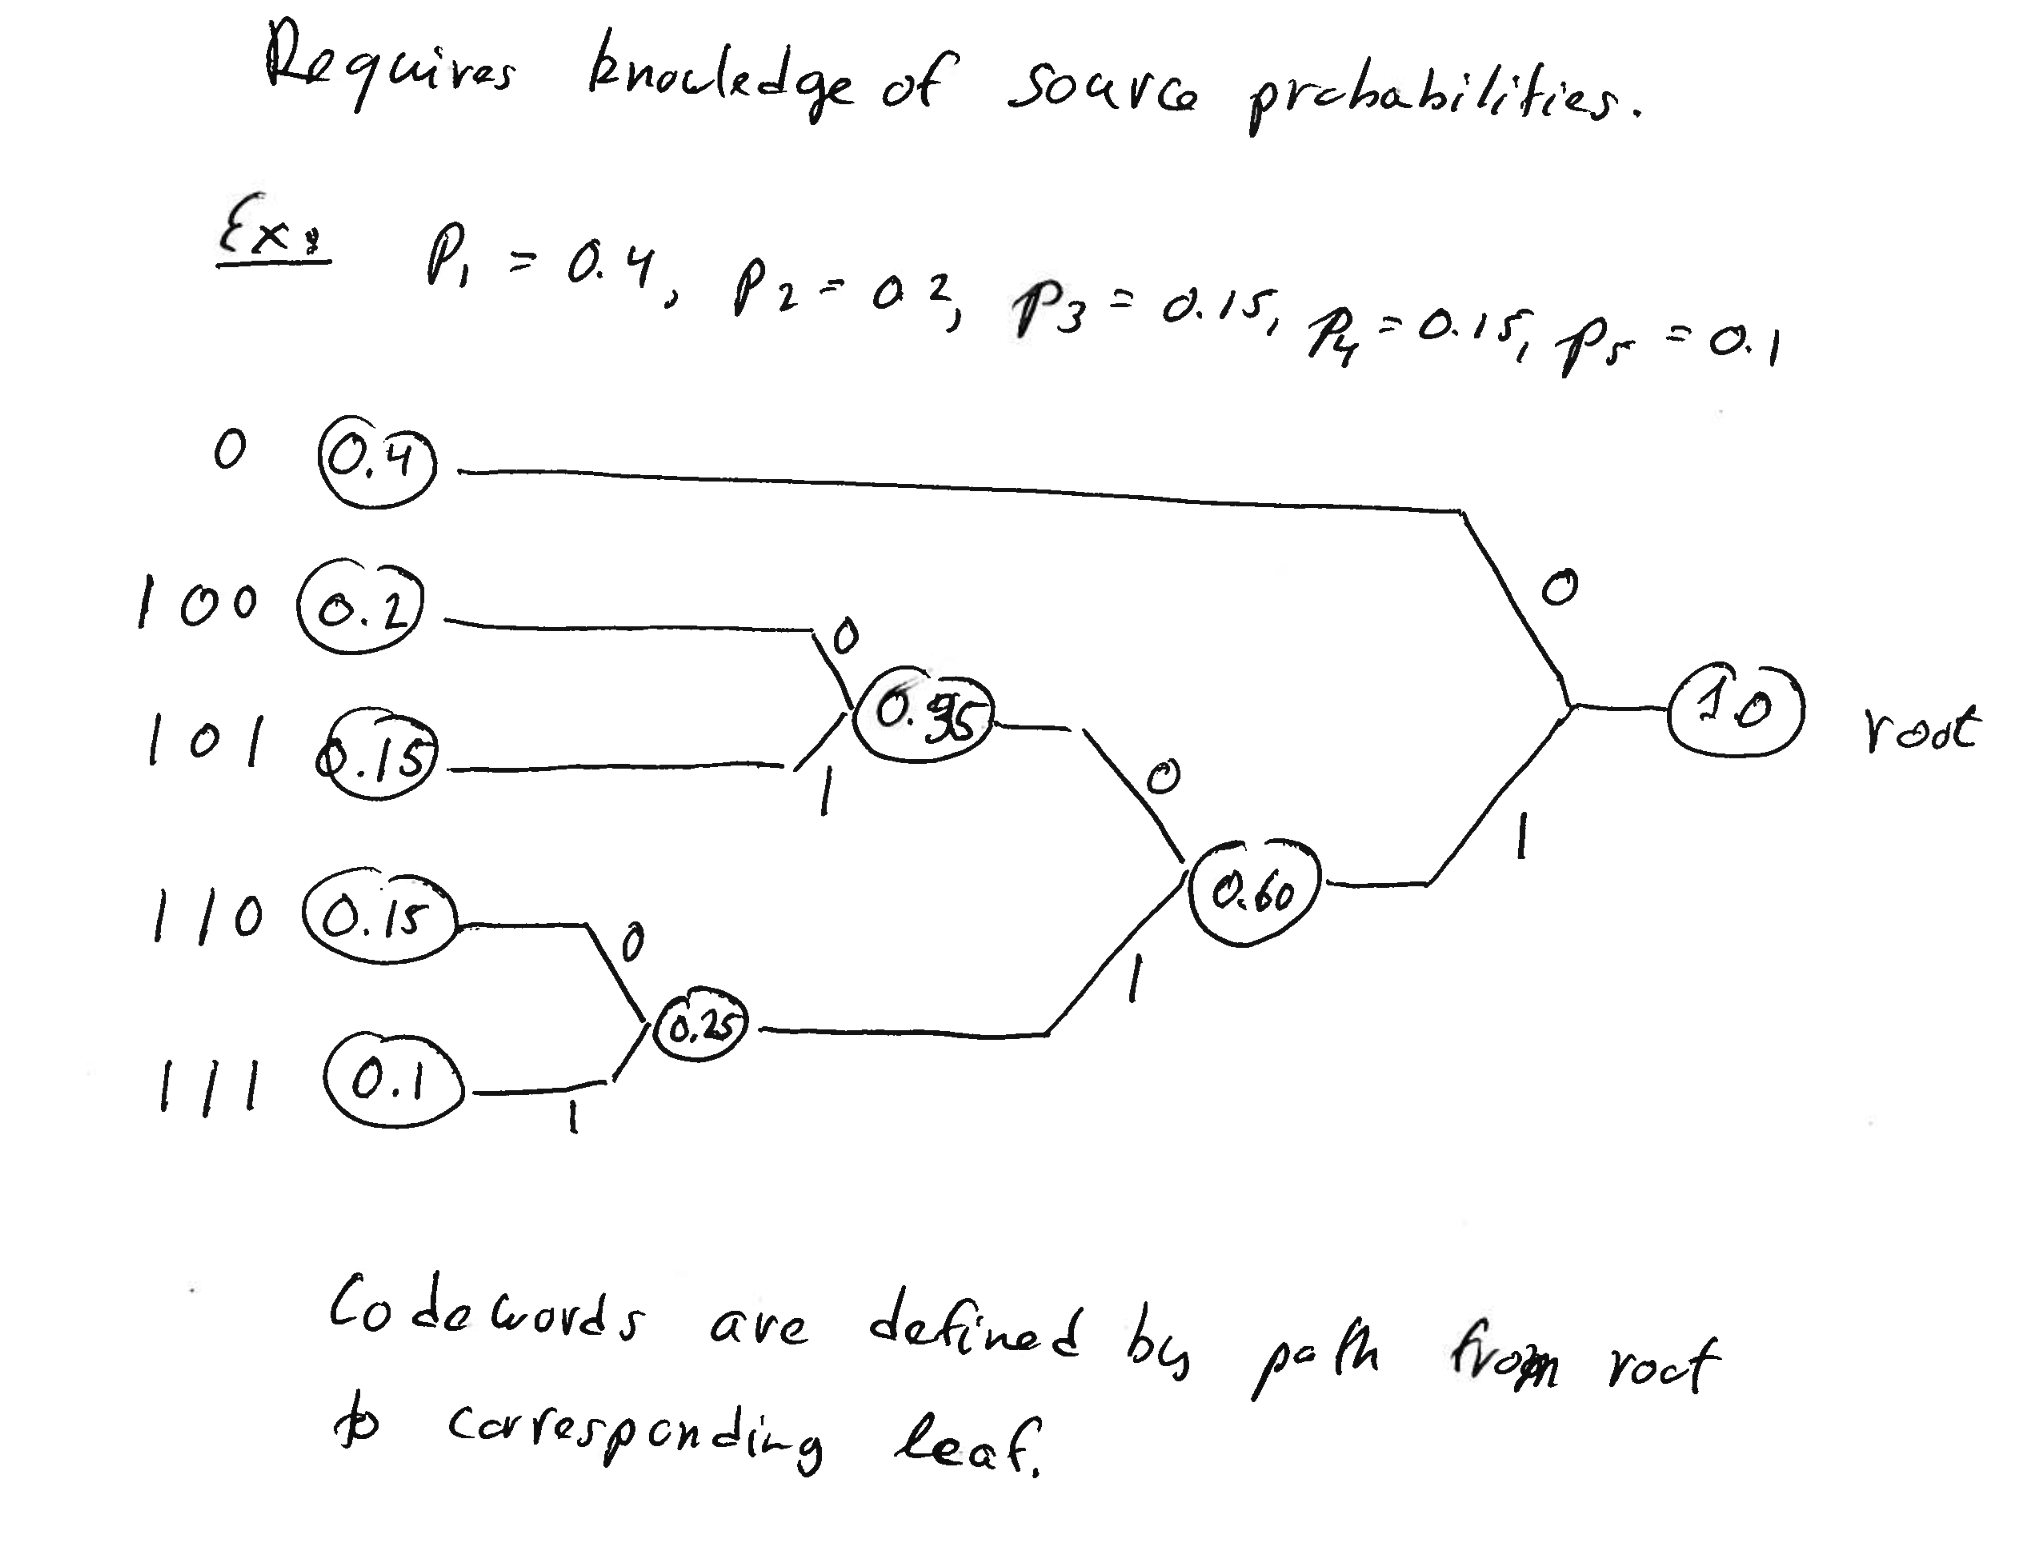
\includegraphics[width=0.5\textwidth]{./img/huffman-example.png}

\section{Channel capacity}
    In this section we discuss \textbf{how much information can be transmitted through a noisy channel}

    \begin{definition}
        A discrete channel consists of a discrete set of words $\mathcal{W}$, two sets of symbols $\mathcal{X}, \mathcal{Y}$, an encoder $\mathcal{W} \rightarrow \mathcal{X}$, a decoder $\mathcal{Y} \rightarrow \mathcal{W}$, and a channel described by the conditional distribution $p_{Y \mid X}$:

        \begin{equation*}
            W \rightarrow X \rightarrow Y \rightarrow \hat{W}
        \end{equation*}

        For this section we are only concerned with \textbf{memoryless} channel: given $X_n$, $Y_n$ is independent of all other variables:

        \begin{equation*}
            p_{\mathbf{Y} \mid \mathbf{X}} = \prod_{l=1}^n p_{Y_l \mid X_l}
        \end{equation*}

        For a fixed $p_{Y \mid X}$, \textbf{information channel capacity} is defined by

        \begin{equation*}
            C^I = \max_{p_X} I(p_X; p_{Y \mid X})
        \end{equation*}
    \end{definition}

    \subsection{Channel rate}
    \begin{definition}[(M, n) code]
        An $(M, n)$-code consists of a collection of $M$ words $\mathcal{W}: \norm{\mathcal{W}} = M$, two sets of symbols $\mathcal{X}, \mathcal{Y}$, an encoder $f: \mathcal{W} \rightarrow \mathcal{X}^n$, and a decoder $g: \mathcal{Y}^n \rightarrow \mathcal{W}$
    \end{definition}

    \begin{definition}[Decoding error]
        For a single word $w \in \mathcal{W}$, the \textbf{conditional probability of error} is defined by

        \begin{equation*}
            \lambda_l = P[g(\mathbf{Y}) \neq l \mid \mathbf{X} = f(w)]
        \end{equation*}

        Denote the \textbf{maximal probability of error} across all words by

        \begin{equation*}
            \lambda^(n) = \max_{w \in \mathcal{W}} \lambda_w
        \end{equation*}

        Denote the \textbf{average probability of error} across all words by

        \begin{equation*}
            P_e^{(n)} = \frac{1}{M}\sum_{w \in \mathcal{W}}\lambda_w
        \end{equation*}

        The \textbf{rate of an $(M, n)$-code} denotes the number of bits of information transmitted per channel use:

        \begin{equation*}
            R = \frac{\log(M)}{n}
        \end{equation*}
    \end{definition}

    \begin{definition}[Achievable rate]
        A rate $R > 0$ is \textbf{achievable} if there exists a sequence of $(2^{nR}, n)$-code such that:

        \begin{equation*}
            \lim_{n \rightarrow \infty}\lambda^{(n)} = 0
        \end{equation*}

        The \textbf{capacity} of a channel is the supremum of all achievable rates
    \end{definition}

    \subsection{Jointly typical sequence}
    Let $(\mathbf{X}, \mathbf{Y}) \in \mathcal{X}^n \times \mathcal{Y}^n$ be i.i.d. sequences drawn according to the joint distribution $P_{X, Y}$, then by the weak law of large numbers, $\lim_{n \rightarrow \infty}-\frac{1}{n}\log(p_{X, Y}(\mathbf{x}, \mathbf{y})) = H(X, Y)$. We can define notion of typicality on the joint sequence similar to the notion of typicality on individual sequences

    \begin{definition}[Jointly typical sequence]
        The set of jointly typical sequence $A_\epsilon^{(n)}$ is the set of $(\mathbf{x}, \mathbf{y})$ such that:

        \begin{enumerate}
            \item $\norm{-\frac{1}{n}\log(p_X(\mathbf{x})) - H(X)} \leq \epsilon$
            \item $\norm{-\frac{1}{n}\log(p_Y(\mathbf{y})) - H(Y)} \leq \epsilon$
            \item $\norm{
                -\frac{1}{n}\log(p_{X, Y}(\mathbf{x}, \mathbf{y})) - H(X, Y)
            } \leq \epsilon$
        \end{enumerate}

        In other words, $(\mathbf{x}, \mathbf{y})$ is jointly typical if $\mathbf{x}$ and $\mathbf{y}$ are each individually typical according to their marginal distribution, and $(\mathbf{x}, \mathbf{y})$ is typical according to the joint distribution
    \end{definition}

    \begin{theorem}[Joint asymptotic equipartition property]
        Let $(\mathbf{X}, \mathbf{Y}) \in \mathcal{X}^n \times \mathcal{Y}^n$ be i.i.d. sequences drawn according to $p_{X, Y}$, then

        \begin{enumerate}
            \item $
                \lim_{n \rightarrow \infty}
                P[(\mathbf{X}, \mathbf{Y}) \in A_\epsilon^{(n)}] = 1
            $
            \item $\norm{A_\epsilon^{(n)}} \leq 2^{
                n(H(X, Y) + \epsilon)
            }$
            \item For sufficiently large $n$:
                $$
                \norm{A_\epsilon^{(n)}} \geq (1-\epsilon)2^{n(H(X, Y) - \epsilon)}
                $$
            \item Let $\tilde{\mathbf{X}}$ and $\tilde{\mathbf{Y}}$ be drawn independently from $p_X$ and $p_Y$, then
                $$
                    P[(\tilde{\mathbf{X}}, \tilde{\mathbf{Y}}) \in A_\epsilon^n] 
                    \leq 2^{-n(I(X; Y) - 3\epsilon)}
                $$
            \item Let $\tilde{\mathbf{X}}$ and $\tilde{\mathbf{Y}}$ be drawn independently from $p_X$ and $p_Y$, then for sufficiently large $n$:
                $$
                    P[(\tilde{\mathbf{X}}, \tilde{\mathbf{Y}}) \in A_\epsilon^n] 
                    \geq (1-\epsilon)2^{-n(I(X; Y) + 3\epsilon)}
                $$
        \end{enumerate}
    \end{theorem}

    \begin{proof}
        (1) is the direct consequence of the weak law of large numbers

        (2):
        \begin{equation*}
            \begin{aligned}
                1 &= \sum_{
                    (\mathbf{x}, \mathbf{y}) \in \mathcal{X}^n \times \mathcal{Y}^n
                    } p(\mathbf{x}, \mathbf{y}) \\
                &\geq \sum_{
                    (\mathbf{x}, \mathbf{y}) \in A_\epsilon^{(n)}
                    } p(\mathbf{x}, \mathbf{y}) \\
                &\geq \sum_{
                    (\mathbf{x}, \mathbf{y}) \in A_\epsilon^{(n)}
                    } 2^{-n(H(X, Y) + \epsilon)} \\
                &=  \norm{A_\epsilon^{(n)}} 2^{-n(H(X, Y) + \epsilon)}
            \end{aligned}
        \end{equation*}

        (3): for sufficiently large $n$, $P[(\mathbf{X}, \mathbf{Y}) \in A_\epsilon^{(n)}] \geq 1 - \epsilon$. On the other hand:

        \begin{equation*}
            \begin{aligned}
                P[(\mathbf{X}, \mathbf{Y}) \in A_\epsilon^{(n)}]
                &= \sum_{(\mathbf{x}, \mathbf{y}) \in A_\epsilon}
                    P[(\mathbf{X}, \mathbf{Y}) = (\mathbf{x}, \mathbf{y})] \\
                &\leq \sum_{(\mathbf{x}, \mathbf{y}) \in A_\epsilon}
                    2^{-n(H_{X,Y} - \epsilon)} \\
                &= \norm{A_\epsilon} \cdot
                    2^{-n(H_{X,Y} - \epsilon)} \\
            \end{aligned}
        \end{equation*}

        Putting the two inequalities above together:

        \begin{equation*}
            \norm{A_\epsilon} \cdot 2^{-n(H_{X,Y} - \epsilon)} \geq 1 - \epsilon
        \end{equation*}
        
        (4): consider the probability of $(\tilde{\mathbf{X}}, \tilde{\mathbf{Y}})$ falling into the jointly typical set:
        \begin{equation*}
            \begin{aligned}
                P[(\tilde{\mathbf{X}}, \tilde{\mathbf{Y}}) \in A_\epsilon^{(n)}]
                &= \sum_{(\tilde{\mathbf{x}}, \tilde{\mathbf{y}}) \in A_\epsilon^{(n)}}
                    P[
                        \tilde{\mathbf{X}} = \tilde{\mathbf{x}},
                        \tilde{\mathbf{Y}} = \tilde{\mathbf{y}}
                    ] \\
                &= \sum_{(\tilde{\mathbf{x}}, \tilde{\mathbf{y}}) \in A_\epsilon^{(n)}}
                    P[\tilde{\mathbf{X}} = \tilde{\mathbf{x}}] \cdot
                    P[\tilde{\mathbf{Y}} = \tilde{\mathbf{y}}] \\
                &\leq \sum_{(\tilde{\mathbf{x}}, \tilde{\mathbf{y}}) \in A_\epsilon^{(n)}}
                    2^{-n(H_X - \epsilon)} \cdot 2^{-n(H_Y - \epsilon)} \\
                &= \norm{A} \cdot 2^{-n(H_X - \epsilon)} \cdot 2^{-n(H_Y - \epsilon)} \\
                &\leq 2^{n(H(X, Y) + \epsilon)} 
                    \cdot 2^{-n(H_X - \epsilon)} \cdot 2^{-n(H_Y - \epsilon)}
            \end{aligned}
        \end{equation*}

        (5): Using similar logic as shown above:
        \begin{equation*}
            \begin{aligned}
                P[(\tilde{\mathbf{X}}, \tilde{\mathbf{Y}}) \in A_\epsilon^{(n)}]
                &= \sum_{(\tilde{\mathbf{x}}, \tilde{\mathbf{y}}) \in A_\epsilon^{(n)}}
                    P[
                        \tilde{\mathbf{X}} = \tilde{\mathbf{x}},
                        \tilde{\mathbf{Y}} = \tilde{\mathbf{y}}
                    ] \\
                &= \sum_{(\tilde{\mathbf{x}}, \tilde{\mathbf{y}}) \in A_\epsilon^{(n)}}
                    P[\tilde{\mathbf{X}} = \tilde{\mathbf{x}}] \cdot
                    P[\tilde{\mathbf{Y}} = \tilde{\mathbf{y}}] \\
                &\geq \sum_{(\tilde{\mathbf{x}}, \tilde{\mathbf{y}}) \in A_\epsilon^{(n)}}
                    2^{-n(H_X + \epsilon)} \cdot 2^{-n(H_Y + \epsilon)} \\
                &= \norm{A_e}
                    2^{-n(H_X + \epsilon)} \cdot 2^{-n(H_Y + \epsilon)} \\
                &\geq (1-\epsilon)2^{n(H_{X,Y} - \epsilon)} \cdot
                    2^{-n(H_X + \epsilon)} \cdot 2^{-n(H_Y + \epsilon)}
            \end{aligned}
        \end{equation*}
    \end{proof}

    \subsection{Channel coding theorem}
    \begin{theorem}
        A rate $R$ is achievable if and only if it is below the information channel capacity
    \end{theorem}
    \begin{proof}
        \textit{This is a sketch of proof}
        
        \textbf{First we show that rate below information capacity is achievable}:
        Let $R$ be a rate such that $R < C$, then we can construct a $(2^{nR}, n)$-code through the following procedure:
        \begin{enumerate}
            \item Find some distribution of $p_X$ and $\epsilon > 0$ such that $R = I(p_X;p_{Y \mid X}) - 4\epsilon$
            \item For each $w \in \{1, \ldots, 2^{nR}\}$, the encoding is $f(w) = (x_1(w), x_2(w), \ldots, x_n(w))$ where $x_i(w)$ is i.i.d. sampled from $p_X$
            \item Transmit each symbol $x_i(w)$ according to $p_{Y \mid X}$
            \item Upon receiving $\mathbf{y}$, find some $\hat{w} \in \{1, \ldots, 2^{nR}\}$ such that $(\mathbf{x}, \mathbf{y})$ is jointly typical according to $p_X$ and $p_{Y \mid X}$ (which can be used to compute $p_{X, Y}$ and $p_Y$)
        \end{enumerate}

        For each word $w$, decoding error occurs if and only if one of two scenarios occurs:

        \begin{enumerate}
            \item $(\mathbf{x}(w), \mathbf{y})$ is not jointly typical, in which case no appropriate $\hat{w}$ can be found in the decoding step
            \item there is another $w^\prime \neq w$ such that $(\mathbf{x}(w^\prime), \mathbf{y})$ is also jointly typical
        \end{enumerate}

        The probability of (1) converges to 0 because $\lim_{n \rightarrow \infty}P[(\mathbf{x}, \mathbf{y}) \not \in A_\epsilon^{(n)}] = 0$.

        The probability of (2) converges to 0 because $\mathbf{y}$ is independent of $\mathbf{x}(w^\prime)$. By joint AEP, the probability of independently sampled sequences being jointly typical is at most $2^{-n(I(X; Y) - 3\epsilon)}$, hence:

        \begin{equation*}
            \begin{aligned}
                \sum_{w^\prime \neq w} P[(\mathbf{x}(w^\prime), \mathbf{y}) \in A_\epsilon^{(n)}]
                &= (2^{nR}-1)P[(\mathbf{x}(w^\prime), \mathbf{y}) \in A_\epsilon^{(n)}] \\
                &\leq (2^{nR}-1)2^{-n(I(X; Y) - 3\epsilon)} \\
                &\leq 2^{nR - n(I_{X;Y} - 3\epsilon)} \\
                &= 2^{n(I_{X;Y} - 4\epsilon) - n(I_{X;Y} - 3\epsilon)} \\
                &= 2^{-n\epsilon}
            \end{aligned}
        \end{equation*}

        Which also converges to 0 as $n \rightarrow \infty$

        \textbf{Converse: achievable rates are below information capacity}

        Recall that the channel represents a Markov chain $W \rightarrow \mathbf{X} \rightarrow \mathbf{Y} \rightarrow \hat{W}$. By Fano's inequality, we know that:

        \begin{equation*}
            H(W \mid \hat{W}) \leq h(p_e) + p_e \cdot \log(\norm{\mathcal{W}})
        \end{equation*}

        Consider the mutual information between $W$ and $\hat{W}$:

        \begin{equation*}
            I(W; \hat{W}) = H(W) - H(W \mid \hat{W})
        \end{equation*}

        Assuming that $W$ is uniformly distributed, $H(W) = \log(\norm{\mathcal{W}}) = nR$.

        By the data-processing inequality $I(W; \hat{W}) \leq I(\mathbf{X}; \mathbf{Y})$. By the chain rule of mutual information: $I(\mathbf{X}; \mathbf{Y}) \leq nI(X; Y)$. By the definition of information channel capacity $I(X; Y) \leq C$. Putting everything together, we have

        \begin{equation*}
            nR - nC \leq p_e
        \end{equation*}

        Assuming the rate is achievable, then $\lim_{n \rightarrow \infty}p_e = 0$, which implies $R \leq C$.
    \end{proof}

\section{Differential entropy}
\begin{definition}
    Let $X \in \mathbb{R}$ be a random variable with probability density function $f_X$. The \textbf{differential entropy} of $X$ is defined by

    \begin{equation*}
        h(X) = -\int_{x \in \mathbb{R}} f_X(x)\ln(f_X(x))dx = -E[\ln(f_X(X))]
    \end{equation*}
\end{definition}

Some notable results:

\begin{itemize}
    \item For uniform distribution over $[0, a]$, $f_X(x) = \frac{1}{a}$, $h(X) = \ln(a)$
    \item For $X \sim N(0, \sigma^2)$, $h(X) = \frac{1}{2}\ln(2\pi e \sigma^2)$
    \item For multivariate normal $\mathbf{X} \sim N(\mathbf{0}, K)$, $h(\mathbf{X}) = \frac{1}{2}\log ((2\pi e)^n \det{K})$
    \item For some constant $a$, $h(X + a) = h(X)$
    \item For some constant $a$, $h(aX) = \ln(\norm{a}) + h(X)$
\end{itemize}

\begin{theorem}
    Let $X$ be continuous random variable with $0$ mean and $\sigma^2$ variance, then

    \begin{equation*}
        h(X) \leq \frac{1}{2}\ln(2\pi e \sigma^2)
    \end{equation*}

    Equality is reached if and only if $X$ is Gaussian
\end{theorem}

\section{Gaussian channel}
\begin{definition}[Information channel capacity]
    Let $Y = X + Z$, where $Z \leftsample N(0, \sigma^2)$ and $E[X^2] \leq P$ for some power level constraint $P$. The \textbf{information channel capacity} is defined by

    $$
    C^I = \max_{f_X : E[X^2] \leq P} I(X; Y)
    $$
\end{definition}

\begin{theorem}
    The information channel capacity of a Gaussian channel is

    \begin{equation}
        \max_{f_X: E[X^2] \leq P} I(X; Y) = \frac{1}{2}\log{(1 + \frac{P}{\sigma^2})}
    \end{equation}

    Where $P$ is the power constraint, and $\sigma^2$ is the variance of the Gaussian noise. The maximum is achieved when $X$ follows Gaussian distribution $X \sim N(0, P)$
\end{theorem}

\subsection{Parallel Gaussian Channel}
Suppose for $1 \leq l \leq n$, $Y_l = X_l + Z_l$, where $Z_l \sim N(0, N_l)$ is independent Gaussian noise, then $\mathbf{Y} = (Y_l)_{l=1}^n$ can be seen as the output of $n$ parallel Gaussian channels combined into a single channel. The capacity of the combined channel is

\begin{equation*}
    C = \max_{f_\mathbf{X}}I(\mathbf{X}; \mathbf{Y})
\end{equation*}

The optimal strategy for maximizing the capacity is to make $X_l$ independent and individually Gaussian. If there is a combined power constraint $\sum_{l=1}^nE[X_l^2] \leq P$, then \textit{power should be first given to the channel with the lowest amount of noise until the combined noise + power exceeds the next lowest noise} (\textbf{waterfilling}).

\section{Rate distortion theory}
    \begin{definition}
        For some fixed $p_X$, the \textbf{information rate distortion} is defined by

        $$
        R^I(D) = \min_{p_{\hat{X} \mid X}: E[d(X, \hat{X})] \leq D} I(X; \hat{X})
        $$
    \end{definition}

    \begin{theorem}
        Let $X$ follow $\operatorname{Bernoulli}(p)$, then

        $$
        R(D) = \begin{cases}
            h(p) - h(D)  & \text{When $D < \min(p, 1-p)$} \\
            0   &  \text{otherwise}
        \end{cases}
    $$
    \end{theorem}

    \begin{theorem}
        For $X \leftsample N(0, \sigma^2)$:

        $$
        R(D) = \begin{cases}
            \frac{1}{2}\log(\frac{\sigma^2}{D}) & (D \leq \sigma^2) \\
            0 & \text{otherwise}
        \end{cases}
        $$
    \end{theorem}
\end{document}